\documentclass[14pt]{beamer}
%\usetheme[compress]{Singapore} % Guia no alto, nada mais, degrade azul
\usetheme{Frankfurt} % Guia no alto, nada mais
\usepackage{subfigure}
\usepackage{multirow}

\title{Economically-Efficient\\Data Stream Analysis}
\author{\small{Roberto Oliveira Jr.\\Advisor: Adriano Veloso \\Co-advisor: Wagner Meira Jr.}}
\institute{Computer Science Dept - UFMG - Brazil}
\date{}

\begin{document}

\begin{frame}
\titlepage
\end{frame}

\section{Data Stream Analysis}

\begin{frame}\frametitle{Data Stream}

\begin{itemize}
\item Definition
\begin{itemize}
\item Fast and possible unbounded sequence of data that arrives at time-varying.
\end{itemize}
\item Motivation
\begin{itemize}
\item It allows us to process huge volumes of data.
\end{itemize}
\end{itemize}
\begin{itemize}
\item Problem
\begin{itemize}
\item Automatically extraction of relevant patterns and relations from data that is continuously created.
\begin{itemize}
\item Keep track of data streams is useful for systems monitoring, online social network advertising, etc.
\end{itemize}
\end{itemize}
\end{itemize}

\end{frame}

\begin{frame}\frametitle{Social Networks Streams and Advertising}

{\underline{Superbowl 2013}}

\begin{figure}
\centering
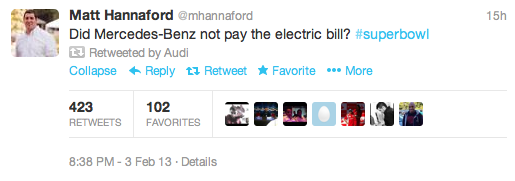
\includegraphics[height=1.30in]{mercedez}
\end{figure}
\vspace{-0.1in}
\begin{figure}
\centering

\includegraphics[height=1.10in]{audi}
\end{figure}

\end{frame}

\begin{frame}\frametitle{Classification in Data Streams}

\begin{itemize}
\item Classification models are applied to distinguish between pre-defined labels.
\end{itemize}

\vspace{-0.2in}
\begin{figure}
\centering
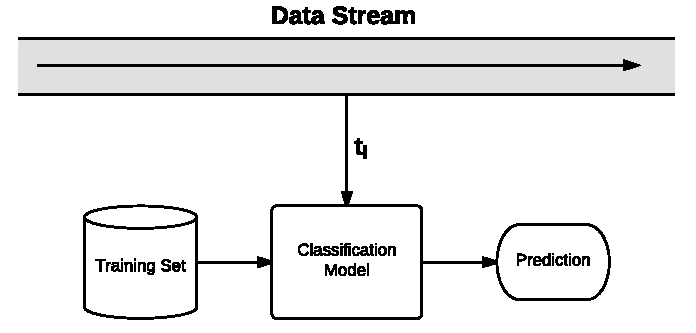
\includegraphics[scale=0.6]{Stream1}
\end{figure}
\vspace{-0.2in}
\pause
\begin{itemize}
\item \alert{Data characteristics may change with time}.
\end{itemize}
\end{frame}

\begin{frame}\frametitle{Concept Drifts}
\begin{itemize}
\item Concept Drift is unforeseen changes in data's nature over time.
\end{itemize}

\vspace{0.1in}
\begin{figure}
\centering
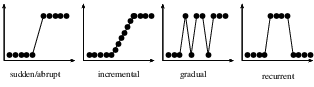
\includegraphics[scale=1]{concept_drift}
\end{figure}
\pause

\begin{itemize}
\item Data streams contains combination of such patterns.
\end{itemize}
\end{frame}


\begin{frame}\frametitle{Sports (WC 2010)}

\vspace{-0.1in}
\begin{figure}
\centering
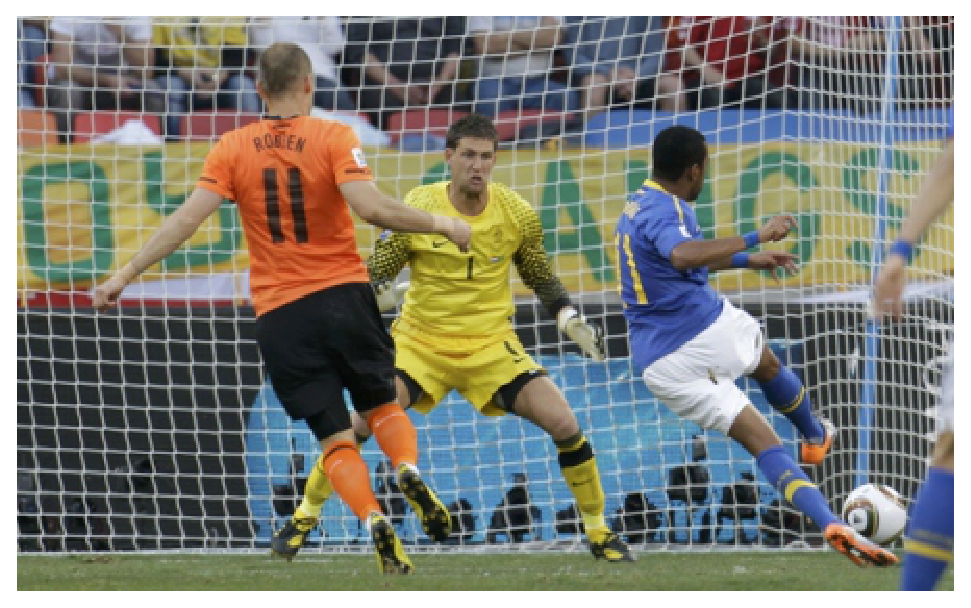
\includegraphics[height=1.00in]{golrobinho.eps}
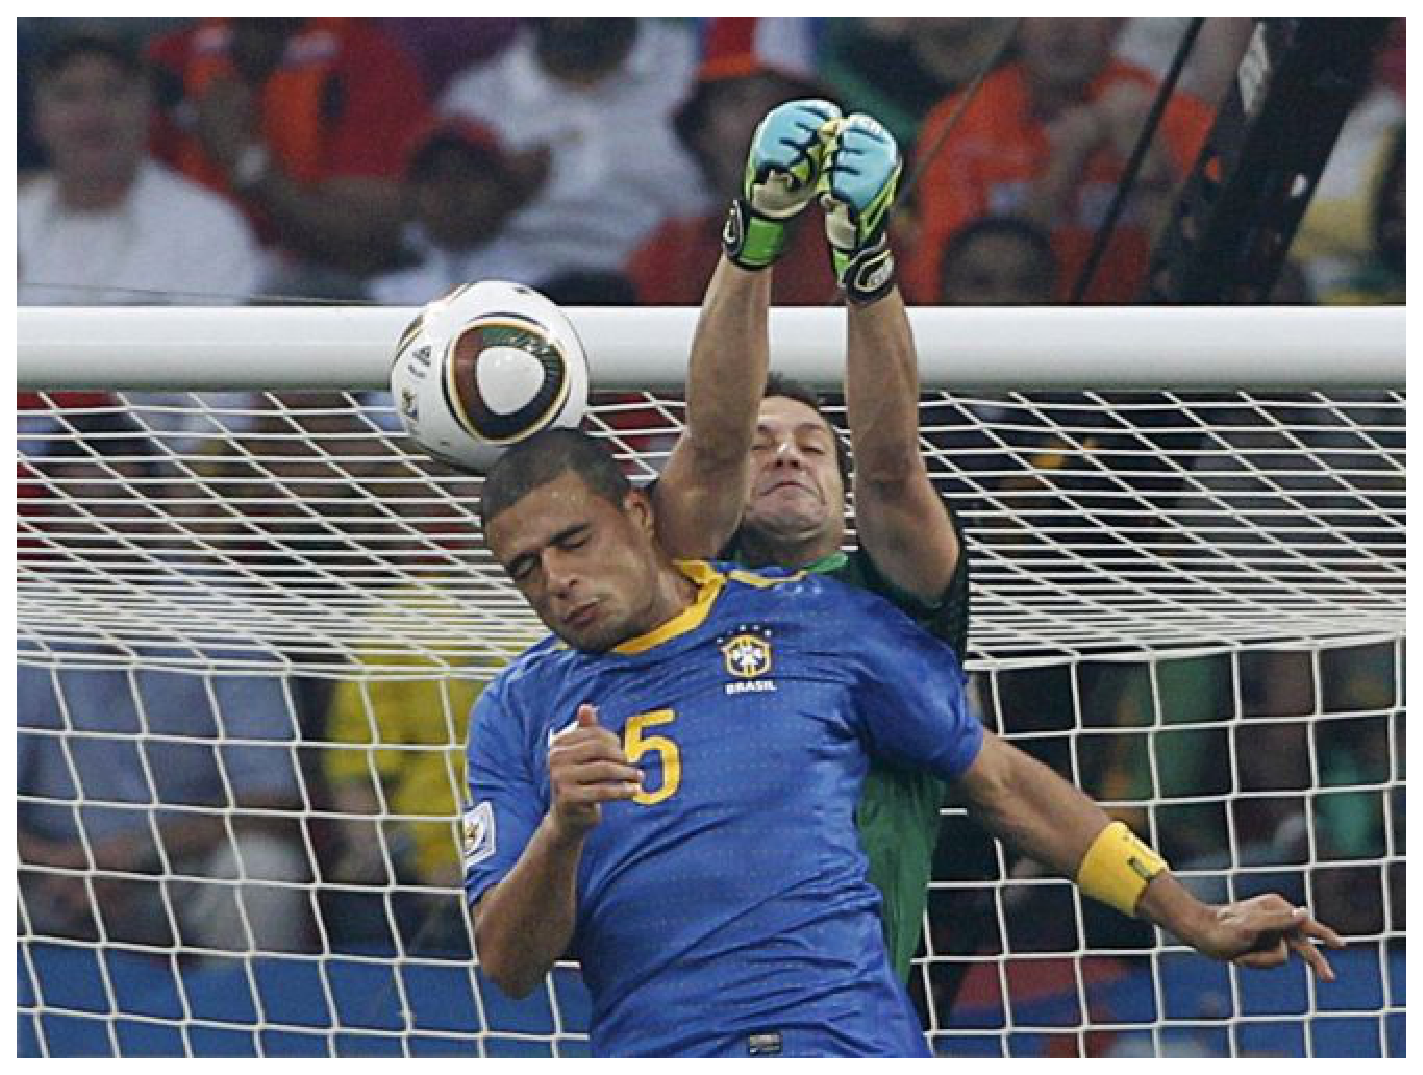
\includegraphics[height=1.00in]{contra.eps}
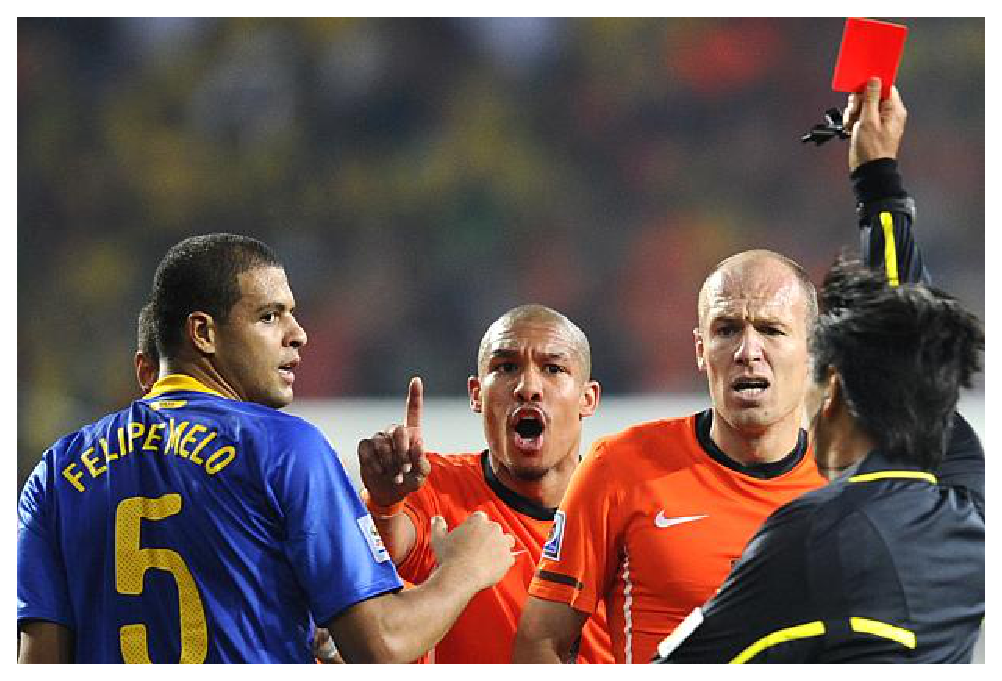
\includegraphics[height=1.00in]{vermelho.eps}
\end{figure}

\vspace{-0.15in}
\begin{figure}
\centering
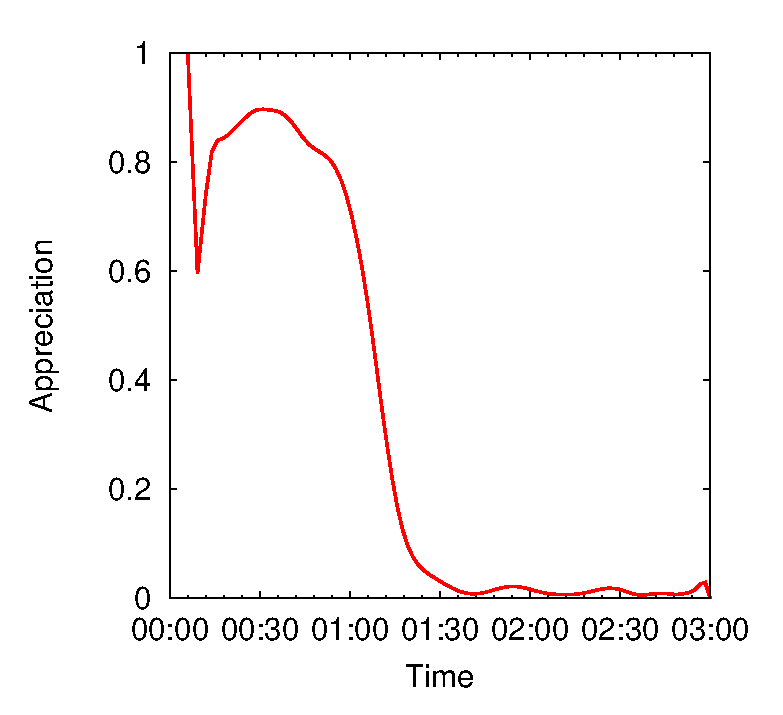
\includegraphics[width=2.35in,height=1.75in]{felipemeloPositividade.eps}
\end{figure}

\end{frame}

\begin{frame}\frametitle{Elections (Brazil 2010)}

\vspace{-0.1in}
\begin{figure}
\centering
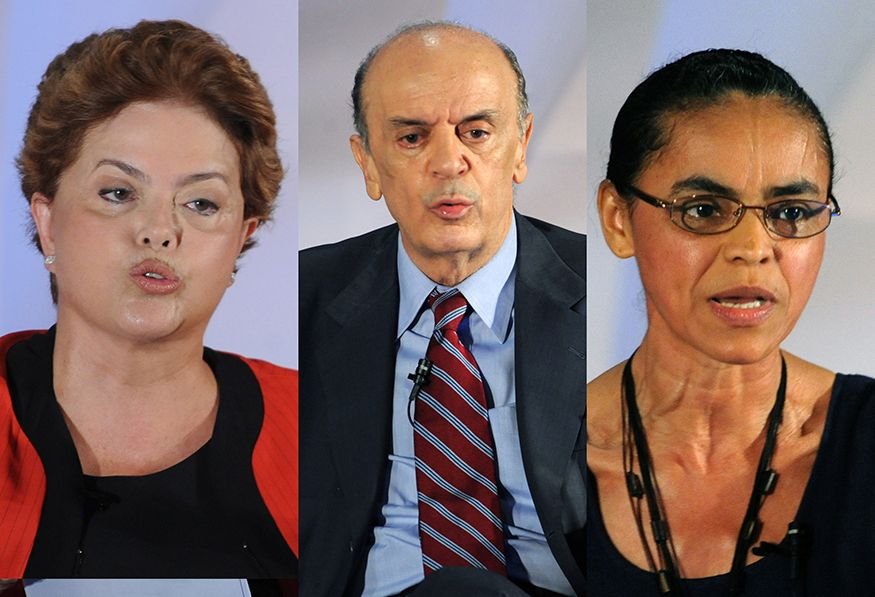
\includegraphics[height=0.95in]{dilma1}
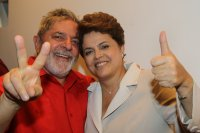
\includegraphics[height=0.95in]{lula}
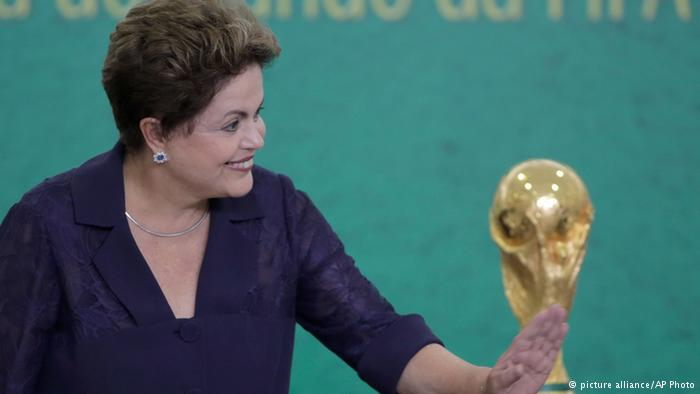
\includegraphics[height=0.95in]{copa}
\end{figure}

\vspace{-0.15in}
\begin{figure}
\centering
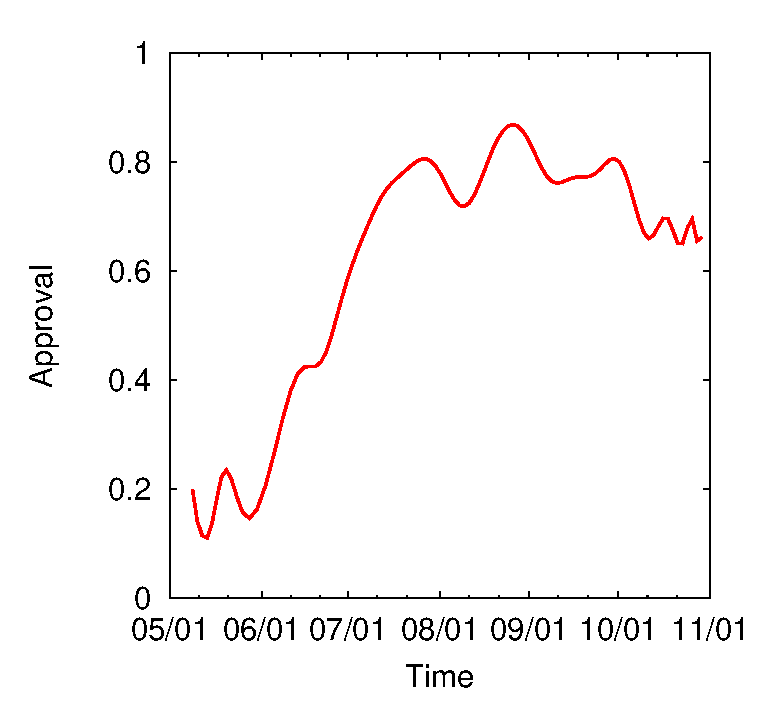
\includegraphics[width=2.35in,height=1.75in]{dilmaPositividade.eps}
\end{figure}

\end{frame}

\begin{frame}\frametitle{Classifying Data Streams}

\begin{itemize}
\item Effective classification requires:
\begin{itemize}
\item Updating the classification model as the stream evolves.
\begin{itemize}
\item Taking into account resources limitation: memory, time and learning requirements.
\end{itemize}
\end{itemize}
\end{itemize}

\vspace{-0.2in}
\begin{figure}
\centering
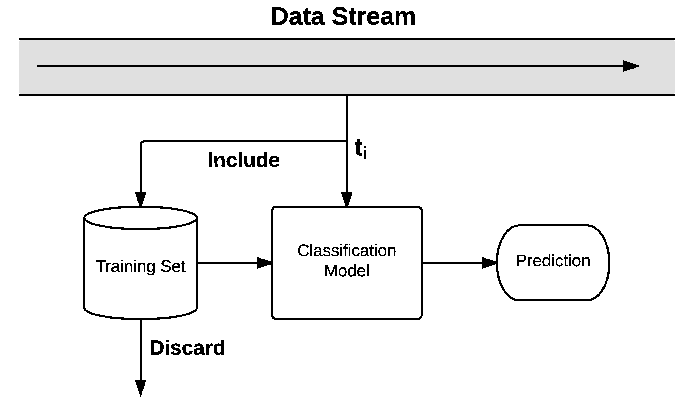
\includegraphics[height=1.60in]{Stream2}
\end{figure}
\end{frame}


\begin{frame}\frametitle{Research Question}

\begin{center}
\large{How to deal with concept drifts?}
\end{center}
% \vspace{0.5in}
% \small{\begin{enumerate}
% \item Which classification model choose?
% \item How to reduce labeling efforts?
% \end{enumerate}}
\end{frame}

\section{Classification Model}
\begin{frame}\frametitle{Classification Model}
\begin{itemize}
\item Classification models are composed by association rules.
  \begin{itemize}
    \item $\{x \to y\}$, where $x \in X$ and $y \in Y$
  \end{itemize}
\item Models are built on-the-fly:
  \begin{itemize}
    \item For a given $[x_i, *]$, rules $\{x \to y\}$ such that $x \in x_i$ are produced.
    \item Prediction is performed from the combination of these rules.
  \end{itemize}
\item At each time step is produced a model $\mathcal{R}(x_i)$.
\pause
\item \alert{Can be updated efficiently as the training set evolves.}
\end{itemize}
\end{frame}

\section{Drifts}
\begin{frame}\frametitle{Dealing with Drifts}

\begin{itemize}
\item Two properties are necessary in order to produce classifiers that are robust to drifts:
\begin{itemize}
\item Adaptiveness:
\begin{itemize}
\item The ability to adapt itself to drifts.
\end{itemize}
\item Memorability:
\begin{itemize}
\item The ability to recover itself from drifts.
\end{itemize}
\end{itemize}
\end{itemize}

\begin{figure}
\centering
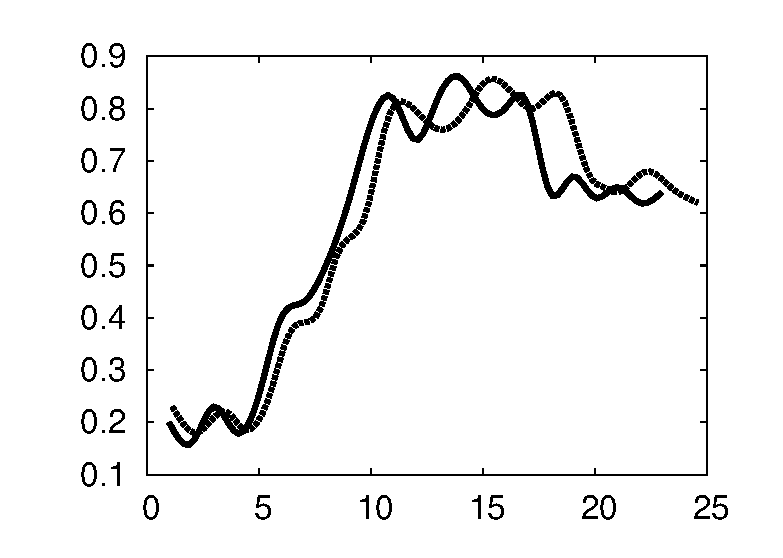
\includegraphics[height=1.30in]{drift3}
\end{figure}
\end{frame}

\begin{frame}\frametitle{Dealing with Drifts}

\begin{itemize}
\item Two properties are necessary in order to produce classifiers that are robust to drifts:
\begin{itemize}
\item Adaptiveness:
\begin{itemize}
\item The ability to adapt itself to drifts.
\item The training-set must contain fresh messages.
\end{itemize}
\item Memorability:
\begin{itemize}
\item The ability to recover itself from drifts.
\item The training-set must contain pre-drift messages.
\end{itemize}
\end{itemize}
\item Improving both properties simultaneously may lead to a conflict-objective problem.
\begin{itemize}
\item Improve adaptiveness may hurt memorability, and vice-versa.
\end{itemize}
\end{itemize}

\end{frame}


\begin{frame}\frametitle{Pareto Efficiency}

Example: hotels in Petr\'{o}polist.

\begin{figure}
\centering
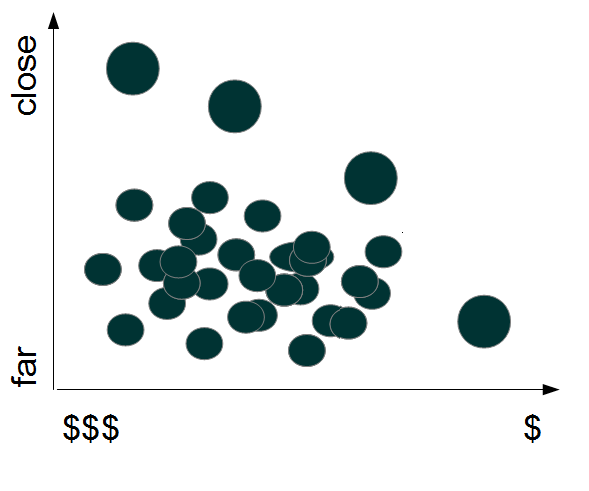
\includegraphics[height=1.60in]{hotel1}
\end{figure}

\end{frame}

\begin{frame}\frametitle{Pareto Efficiency}

Pareto frontier

\begin{figure}
\centering
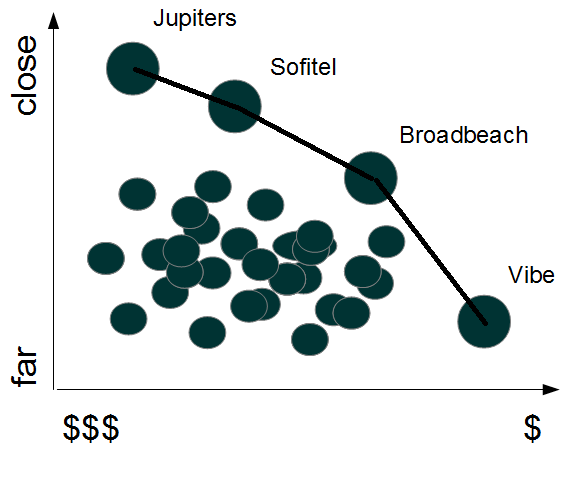
\includegraphics[height=1.60in]{hotel2}
\end{figure}

\end{frame}

\begin{frame}\frametitle{Compensation $-$ Kaldor-Hicks Principle}

Region of compensation

\begin{figure}
\centering
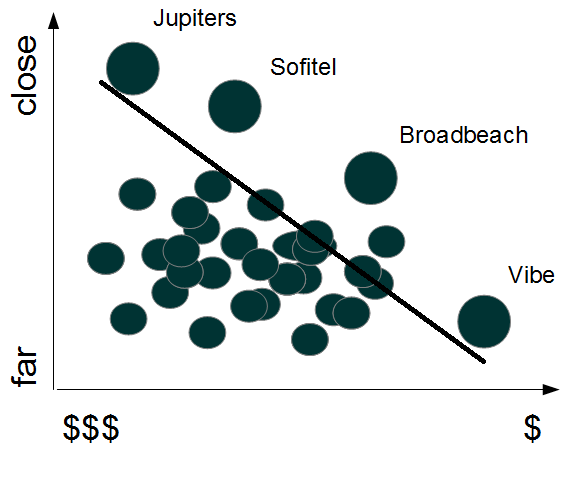
\includegraphics[height=1.60in]{hotel3}
\end{figure}

\end{frame}

\begin{frame}\frametitle{Utility Measures}
\begin{itemize}
\item Distance in space:
\begin{itemize}
\item How similar message $t_j$ is to the newest message $t_n$.
\item $U_s(t_j)=\frac{|\mathcal{R}(t_n) \cap \mathcal{R}(t_j)|}{|\mathcal{R}(t_n)|}$
\end{itemize}
\item Distance in time:
\begin{itemize}
\item How fresh is the message.
\item $U_t(t_j)=\frac{\gamma(t_j)}{\gamma(t_n)}$.
\begin{itemize}
\item $\gamma(t_j)$ returns the time in which message $t_j$ arrived.
\end{itemize}
\end{itemize}
\item Random permutation of messages:
\begin{itemize}
\item $U_r(t_j)=\frac{\alpha(t_j)}{|\mathcal{D}_n|}$
\begin{itemize}
\item $\alpha(t_j)$ returns the position of $t_j$ in the shuffle.
\item $\mathcal{D}_n$ is the training set at time step $n$.
\end{itemize}
\end{itemize}
\end{itemize}

\end{frame}

\begin{frame}\frametitle{Utility Measures}

\begin{enumerate}
\item At each time step $n$:
\begin{enumerate}
\item Place candidate messages in the utility space.
\item Select messages in the Efficiency Region (Pareto-frontier / Kaldor-Hicks Region).
\end{enumerate}
\end{enumerate}

\vspace{-0.1in}
\begin{figure}
\centering
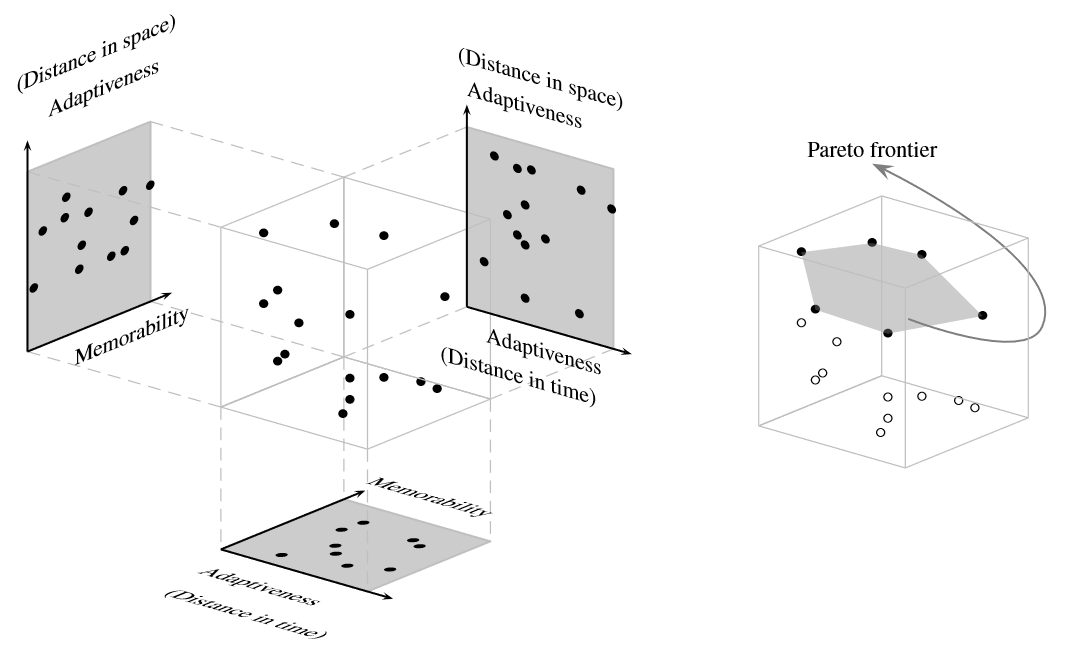
\includegraphics[height=2.30in]{pareto}
\end{figure}

\end{frame}

\section{Labeling Efforts}
\begin{frame}\frametitle{Reducing Labeling Efforts}
\begin{itemize}
\item Random Active Learning
\begin{itemize}
\item Naive strategy.
\item Simple to integrate.
\item Labeling Effort control: $\delta$.
\end{itemize}
\end{itemize}
\end{frame}

\section{Economically-Efficient Data Stream Analysis}
\begin{frame}\frametitle{EESS in Stream Classification Flow}
\begin{figure}
\centering
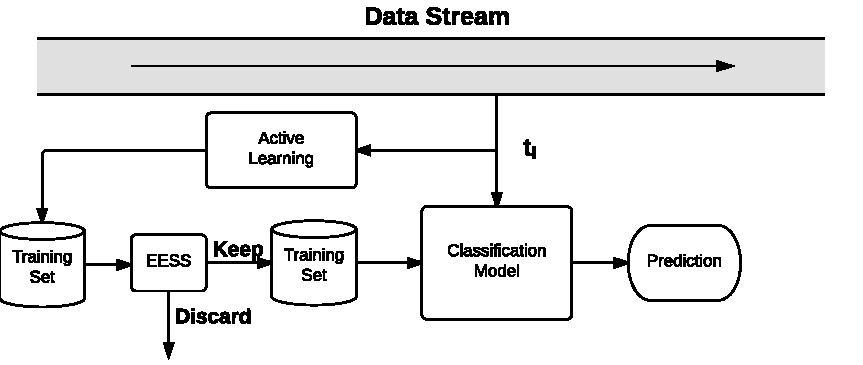
\includegraphics[scale=0.7]{EESS}
\end{figure}
\end{frame}

\section{Results}
\begin{frame}
\frametitle{Experimental Evaluation}
\framesubtitle{Setup}
\begin{itemize}
    \item Interleaved Test-Then-Train
    \item 1\% of data provided as training seed;
    \item Massive Online Analysis (MOA) framework as evaluation environment;
    \item Baselines:
    \begin{itemize}
      \item AC $-$ Active Classifiers (KDD 2011)
      \item HAT $-$ Hoeffding Adaptive Trees (JMLR 2011)
      \item ILAC $-$ Incremental Lazy Classifiers (SIGIR 2011)
    \end{itemize}
    \item Labeling Efforts (AC and EESS): 10\%; \textbf{25\%}; 50\%; 75\% and 100\%;
\end{itemize}

\end{frame}

\begin{frame}\frametitle{Evaluation}

\begin{itemize}
\item Measures used:
\begin{itemize}
\item Mean Squared Error.
\item Labeling Effort.
\item Training set site.
\item RAM-Hours:
\begin{itemize}
\item A GB of RAM deployed for 1 hour execution.
\end{itemize}
\end{itemize}
\item Datasets:
\end{itemize}
\begin{table}
\centering
\scalebox{0.7}{
\begin{tabular}{lcccc}
\hline
& \multicolumn{4}{c}{Concept Drift Pattern} \\ \cline{2-5}
Dataset & Sudden & Incremental & Gradual & Recurrent \\
\hline \hline
Presidential Elections & - & X & X & - \\
Person of the Year & - & X & X &  - \\
\textbf{FIFA World Cup - EN} & X & - & - & - \\
\textbf{FIFA World Cup - PT} & X & - & - & -  \\
\textbf{Cover Type} & X & - & X & X \\
Spam Filtering & X & - & X & X \\
\textbf{Poker Hand} & - & - & X & X \\
\hline
\end{tabular}
}
\end{table}
\end{frame}

% \begin{frame}\frametitle{Datasets}
% \begin{itemize}
% \item Seven datasets from different applications:
% \begin{itemize}
% \item Sentiment Analysis
% \item Forest cover type prediction
% \item Spam filtering
% \item Poker game
% \end{itemize}
% \end{itemize}

% \end{frame}

\begin{frame}
\frametitle{Evaluation}
\framesubtitle{Brazilian Presidential Elections}
MSE and Labeling Efforts
\begin{figure}[htp!]
\label{fig:dilma_1}
\centering
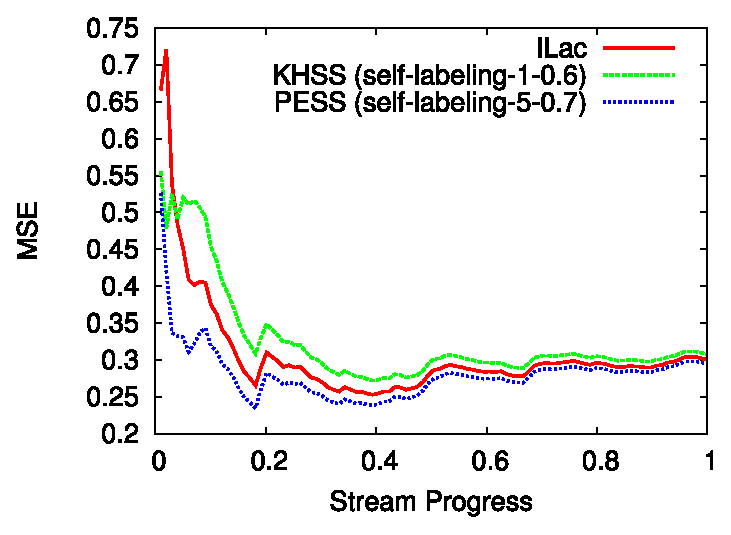
\includegraphics[scale=0.41]{dilma_mse.eps}
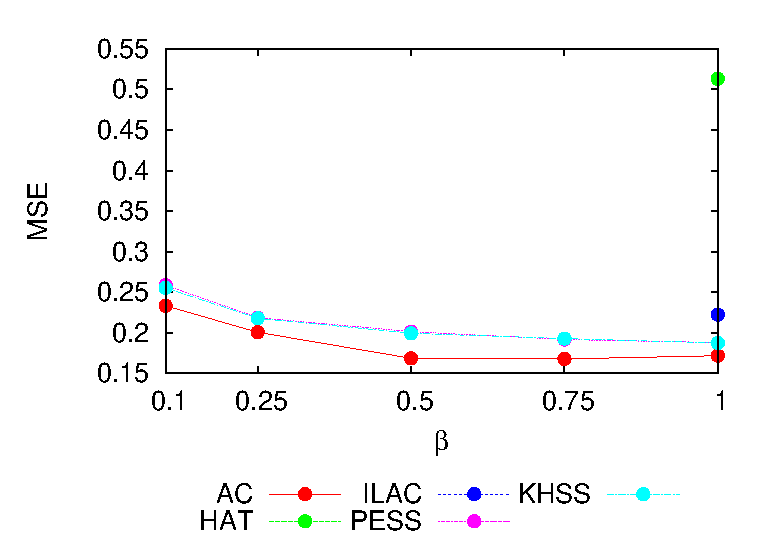
\includegraphics[scale=0.41]{dilma_le_mse.eps}
\end{figure}
\end{frame}

\begin{frame}
\frametitle{Evaluation}
\framesubtitle{Brazilian Presidential Elections}
Training Size and RAM-Hours
\begin{figure}[htp!]
\label{fig:dilma_2}
\centering
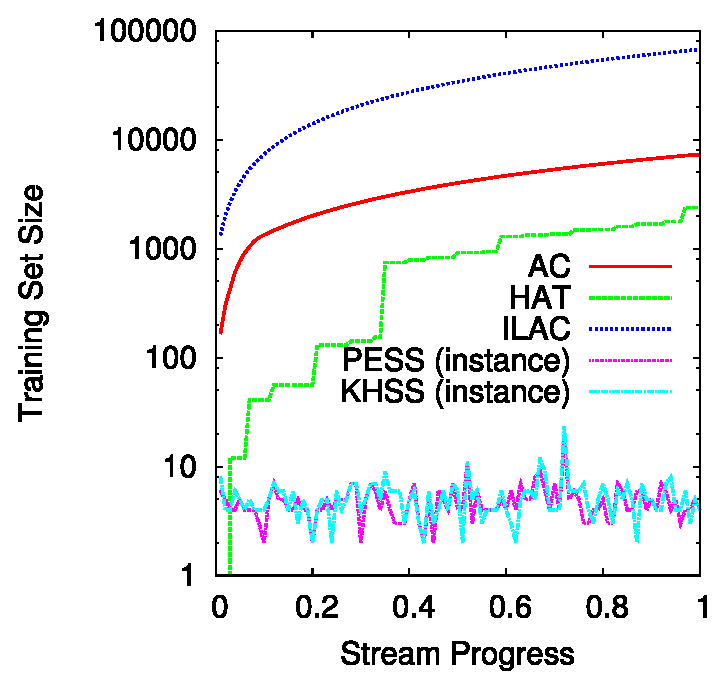
\includegraphics[scale=0.41]{dilma_window.eps}
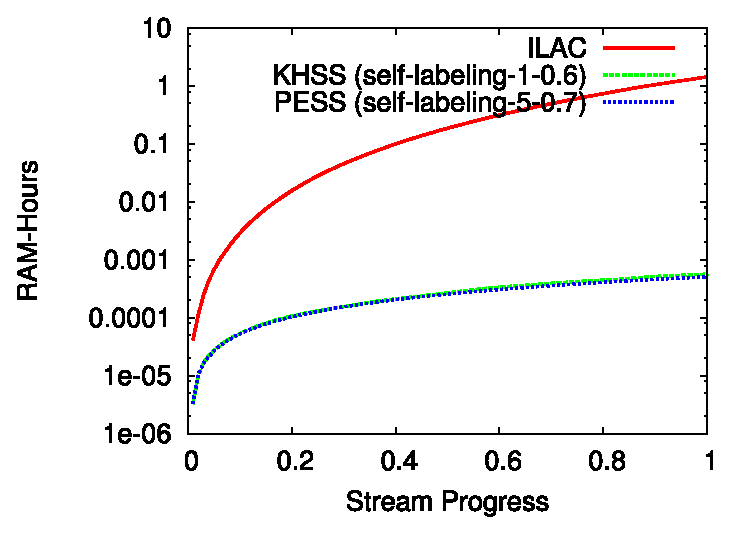
\includegraphics[scale=0.41]{dilma_ramhours.eps}
\end{figure}
\end{frame}

\begin{frame}
\frametitle{Evaluation}
\framesubtitle{FIFA World Cup - Portuguese}
MSE and Labeling Efforts
\begin{figure}[htp!]
\label{fig:fm_1}
\centering
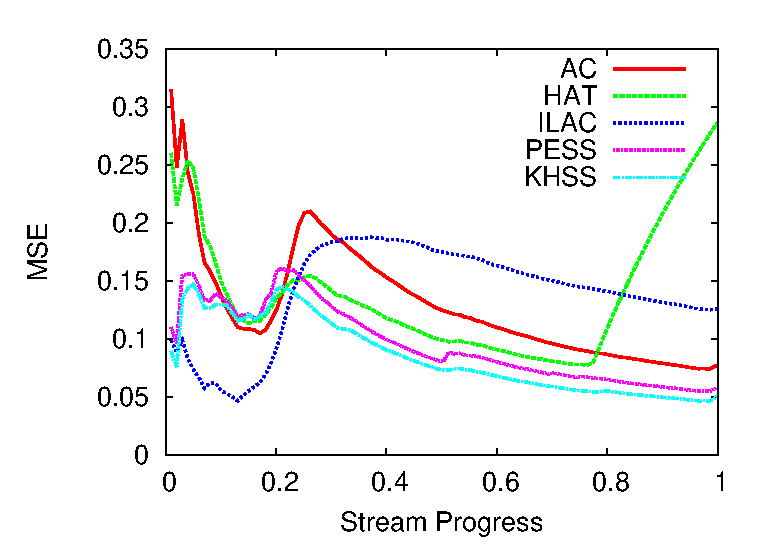
\includegraphics[scale=0.41]{pt_mse.eps}
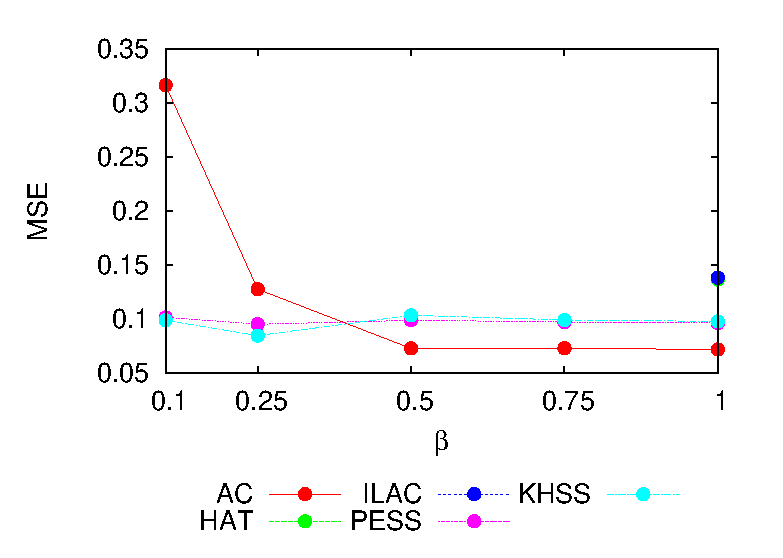
\includegraphics[scale=0.41]{pt_le_mse.eps}
\end{figure}
\end{frame}

\begin{frame}
\frametitle{Evaluation}
\framesubtitle{FIFA World Cup - Portuguese}
Training Size and RAM-Hours
\begin{figure}[htp!]
\label{fig:fm_2}
\centering
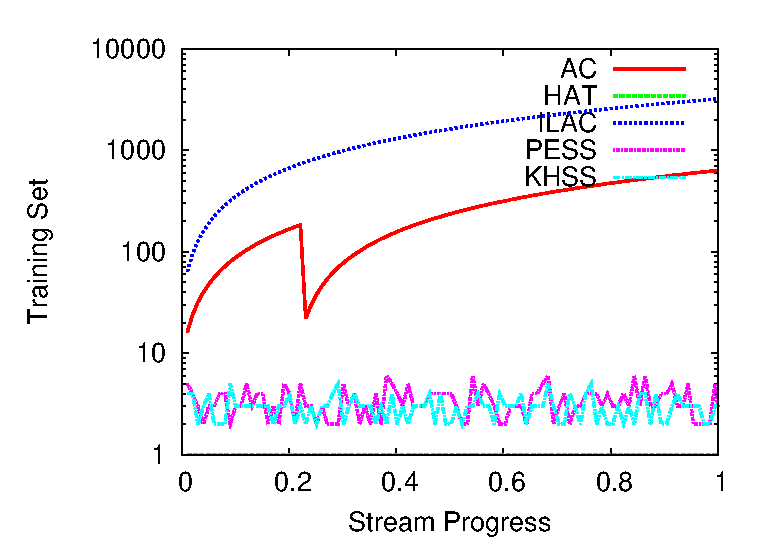
\includegraphics[scale=0.41]{pt_window.eps}
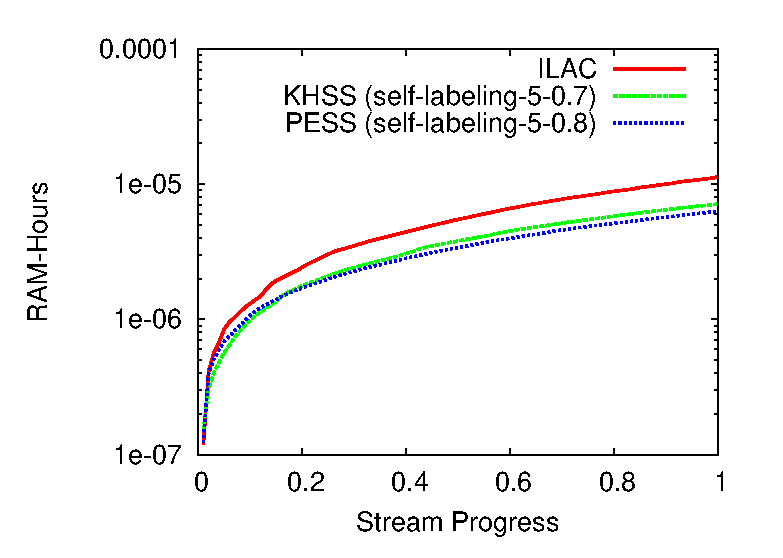
\includegraphics[scale=0.41]{pt_ramhours.eps}
\end{figure}
\end{frame}

\section{Conclusions}

\begin{frame}\frametitle{Conclusions}

\begin{itemize}
\item Sentiment analysis on Twitter streams.
\begin{itemize}
\item Limited computing and training resources.
\item Sentiment drifts.
\end{itemize}
\item Efficiency and accuracy.
\begin{itemize}
\item Incremental classifiers.
\item Pareto efficiency and compensation principle.
\end{itemize}
\item Our results.
\begin{itemize}
\item 50\% reduction in terms of labeling effort without impact on accuracy.
\end{itemize}
\item Future work includes:
\begin{itemize}
\item Other utility measures.
\item Other application scenarios.
\end{itemize}
\end{itemize}

\end{frame}

\section{Contact}
\begin{frame}{Thank you!}
\begin{center}
\tt adrianov@dcc.ufmg.br\\
\end{center}
\end{frame}

\end{document}


